\begin{frame}{Không gian \(\mathcal{X}\)}
    \begin{center}
        \begin{minipage}{0.4\linewidth}
            \begin{center}
                \resizebox{1\linewidth}{!}{


\tikzset{every picture/.style={line width=0.75pt}} %set default line width to 0.75pt        

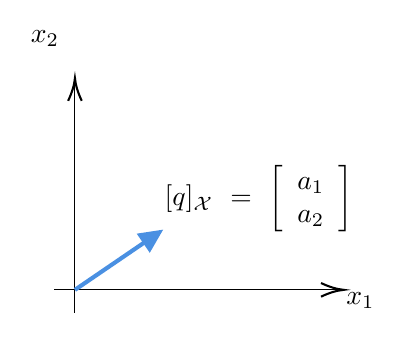
\begin{tikzpicture}[x=0.75pt,y=0.75pt,yscale=-1,xscale=1]
%uncomment if require: \path (0,15225); %set diagram left start at 0, and has height of 15225

%Straight Lines [id:da30187225832710496] 
\draw    (283,3620) -- (420.5,3620) ;
\draw [shift={(422.5,3620)}, rotate = 180] [color={rgb, 255:red, 0; green, 0; blue, 0 }  ][line width=0.75]    (10.93,-3.29) .. controls (6.95,-1.4) and (3.31,-0.3) .. (0,0) .. controls (3.31,0.3) and (6.95,1.4) .. (10.93,3.29)   ;
%Straight Lines [id:da7150609245229815] 
\draw    (293,3631) -- (293,3620) -- (293,3520) ;
\draw [shift={(293,3518)}, rotate = 90] [color={rgb, 255:red, 0; green, 0; blue, 0 }  ][line width=0.75]    (10.93,-3.29) .. controls (6.95,-1.4) and (3.31,-0.3) .. (0,0) .. controls (3.31,0.3) and (6.95,1.4) .. (10.93,3.29)   ;
%Straight Lines [id:da12230210739845826] 
\draw [color={rgb, 255:red, 74; green, 144; blue, 226 }  ,draw opacity=1 ][line width=1.5]    (293,3620) -- (332.2,3593.25) ;
\draw [shift={(335.5,3591)}, rotate = 145.69] [fill={rgb, 255:red, 74; green, 144; blue, 226 }  ,fill opacity=1 ][line width=0.08]  [draw opacity=0] (11.61,-5.58) -- (0,0) -- (11.61,5.58) -- cycle    ;

% Text Node
\draw (422.5,3620) node [anchor=north west][inner sep=0.75pt]    {$x_{1}$};
% Text Node
\draw (270.5,3494) node [anchor=north west][inner sep=0.75pt]    {$x_{2}$};
% Text Node
\draw (335,3559) node [anchor=north west][inner sep=0.75pt]    {$[ q]_{\mathcal{X}} \ =\ 
\left[
\begin{array}{c}
a_1 \\ a_2
\end{array} \right] $};


\end{tikzpicture}}
            \end{center}
        \end{minipage}
        \hspace{1mm}
        \begin{minipage}{0.4\linewidth}
            Gọi \(q\) là một vector trong không gian \(\mathcal{X}\). \(q\) là một tổ hợp tuyến tính 
            \begin{equation}
                q = \sum_{i=1}^{2} a_i x_i.
                \label{eq:3.2}
            \end{equation}
        \end{minipage}
    \end{center}
\end{frame}